\documentclass[12pt,a4paper,table]{article}

\usepackage[a4paper,
            tmargin=2cm,
            bmargin=2cm,
            lmargin=2cm,
            rmargin=2cm,
            bindingoffset=0cm]{geometry}

\usepackage{lmodern}
\usepackage[T1]{polski}
\usepackage[utf8]{inputenc}
\usepackage{tocloft}
\usepackage{hyperref}
\usepackage{amsmath}
\usepackage{listings}
\usepackage{graphicx}
\usepackage{subfig}
\usepackage{float}
\usepackage{booktabs}

\hypersetup{
    colorlinks,
    citecolor=black,
    filecolor=black,
    linkcolor=black,
    urlcolor=black
}

\newtheorem{definition}{Def}


\begin{document}
    \title {
        Teaoria współbieżności

    }

    \author{
        Przemysław Węglik
    }

    \date{\today}

    \maketitle

    \section{Opis eksperymentu}

    Dla stałego czasu $t = 1s$, uruchamiamy $p$ producentów i 
    $k$ konsumentów przy czym w analizach poniżej $p = k$.
    
    Po minięciu czasu $t$ zatrzymujemy wszystkie wątki i zliczamy
    sumaryczny czas CPU, ilość wykonanych operacji jednostkowych
    na współdzielonym bufforze, a także ilość operacji w czasie 
    jednej sekundy pracy CPU.

    \section{Wyniki}

    Poniżej przedstawiono wykresy czas CPU i 
    ilość wykonanych operacji jednostkowych w zależności od
    łącznej liczby wątków ($p + k$)

    \subsection{Rozwiązanie przy użyciu 4 Conditions}
    \begin{figure}[H]
        \centering
        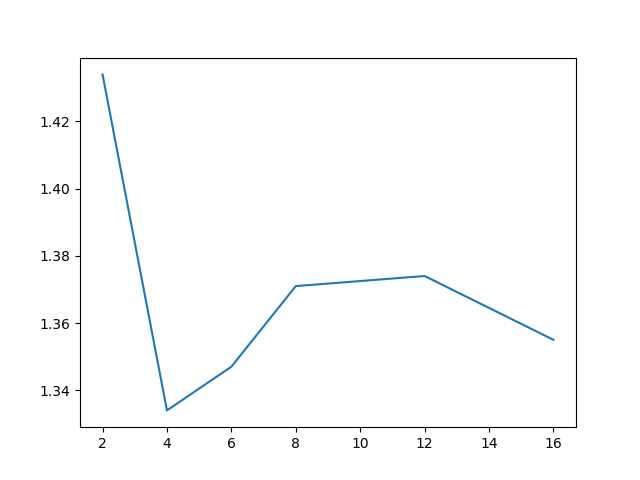
\includegraphics[width=0.6\linewidth]{img/4_cond_cpu.png}
        \caption{Wykres czasu CPU od liczby wątków}
        \label{fig:4_cond_cpu}
    \end{figure}

    \begin{figure}[H]
        \centering
        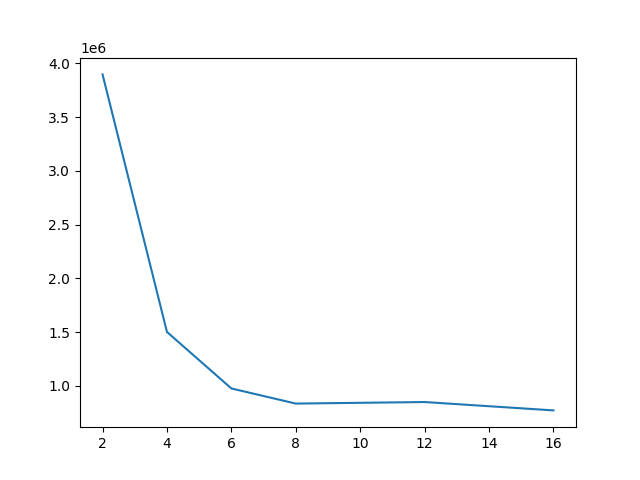
\includegraphics[width=0.6\linewidth]{img/4_cond_count.png}
        \caption{Wykres operacji jednostkowych na bufforze od liczby wątków}
        \label{fig:4_cond_cpu}
    \end{figure}

    \begin{figure}[H]
        \centering
        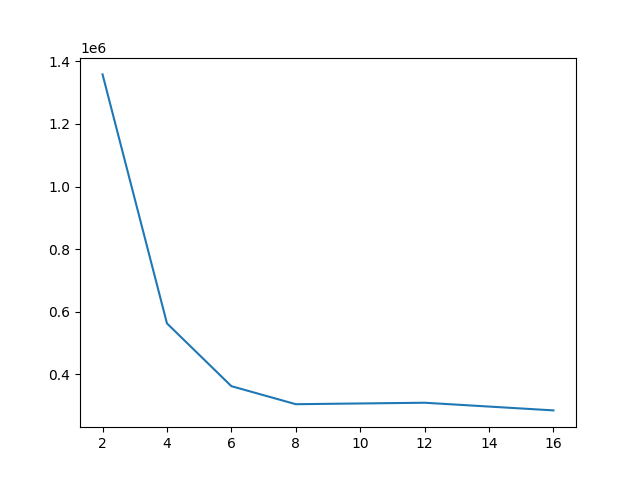
\includegraphics[width=0.6\linewidth]{img/4_cond_count_per_cpu.png}
        \caption{Wykres operacji jednostkowych w sekundzie czasu CPU od liczby wątków}
        \label{fig:4_cond_cpu}
    \end{figure}

    \subsection{Rozwiązanie przy użyciu zagnieżdżonych Locków}

    \begin{figure}[H]
        \centering
        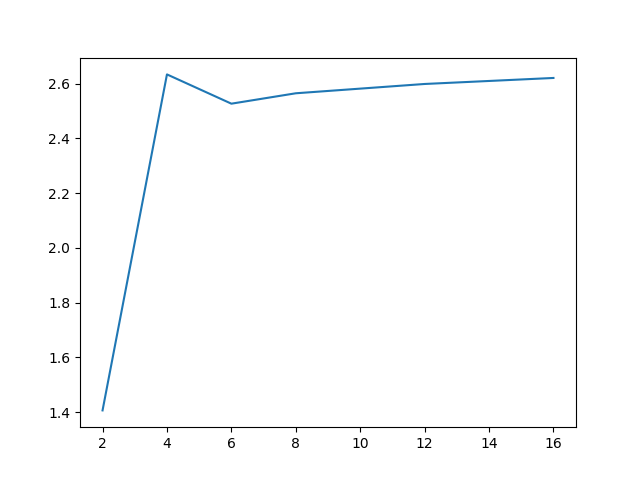
\includegraphics[width=0.6\linewidth]{img/lock_cpu.png}
        \caption{Wykres czasu CPU od liczby wątków}
        \label{fig:lock_cpu}
    \end{figure}

    \begin{figure}[H]
        \centering
        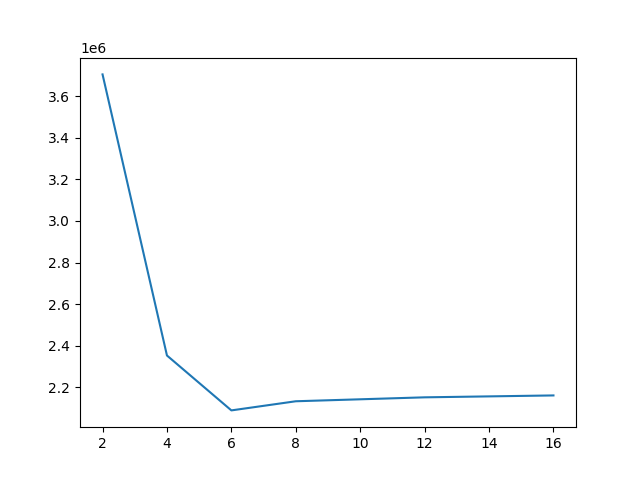
\includegraphics[width=0.6\linewidth]{img/lock_count.png}
        \caption{Wykres operacji jednostkowych na bufforze od liczby wątków}
        \label{fig:lock_count}
    \end{figure}

    \begin{figure}[H]
        \centering
        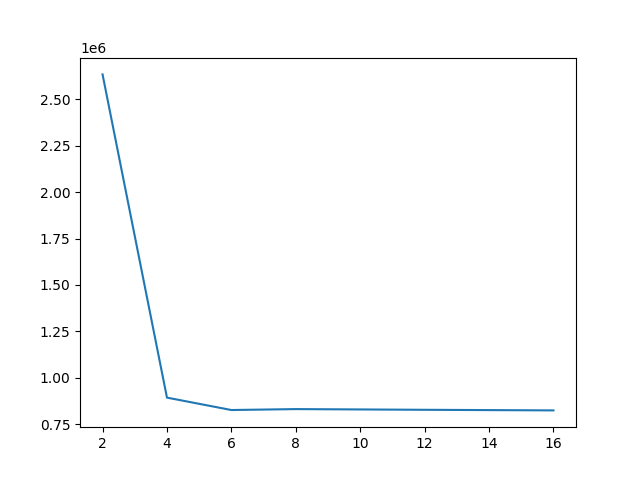
\includegraphics[width=0.6\linewidth]{img/lock_count_per_cpu.png}
        \caption{Wykres operacji jednostkowych w sekundzie czasu CPU od liczby wątków}
        \label{fig:lock_count_per_cpu}
    \end{figure}

    \section{Omówienie wyników}
    Rozwiązanie przy użyciu 4 Conditions zużywało średnio około 2 razy
    mniej czasu procesora, ale przetworzyło ponad 50\% mniej 
    danych w tym samym czasie rzeczywistym.



\end{document}